\documentclass[11pt,a4paper]{article}
\usepackage[utf8]{inputenc}
\usepackage{color}
\usepackage{enumerate}
\usepackage{fancyhdr}
\usepackage{minted}
\usepackage{graphicx}
\usepackage{array}
\usepackage{hyperref}
\usepackage[spanish]{babel}
\usepackage[spanish]{algorithm2e}

\setlength{\oddsidemargin}{18pt}
\setlength{\headheight}{14pt}
\setlength{\textheight}{609pt}
\setlength{\marginparsep}{11pt}
\setlength{\footskip}{30pt}
\hoffset = 0pt
\voffset = 0pt
\setlength{\topmargin}{0pt}
\setlength{\headsep}{25pt}
\setlength{\textwidth}{424pt}
\setlength{\marginparwidth}{54pt}
\setlength{\marginparpush}{5pt}
\paperwidth = 597pt
\paperheight = 845pt

\pagestyle{fancy}
\fancyhead[LO]{\textcolor[rgb]{0,0,0}{Grado en Ingeniería Informática}}
\fancyhead[RO]{\textcolor[rgb]{0.2,0.2,0.9}{Algorítmica, Curso 2015-2016}}

\hypersetup{
	colorlinks,
	citecolor=black,
	filecolor=black,
	linkcolor=black,
	urlcolor=black
}

\newmintedfile[BusquedaFB]{c++}{
	%linenos,
	firstline=16,
	lastline=36,
	numbersep=5pt,
	gobble=0,
	frame=lines,
	framesep=2mm,
	tabsize=3,
}

\newmintedfile[BusquedaDyV]{c++}{
	%linenos,
	firstline=38,
	lastline=60,
	numbersep=5pt,
	gobble=0,
	frame=lines,
	framesep=2mm,
	tabsize=3,
}


\begin{document}

	\begin{titlepage}

		\centering

		\begin{figure}[h]

			\centering
			
\includegraphics[width=0.6\textwidth]{logo-ugr.png}
			
		\end{figure}

		\vspace{1cm}

		{\scshape\LARGE Universidad de Granada}

		\vspace{1cm}

		{\LARGE Algorítmica}

		\vspace{1cm}

		{\huge\bfseries\textit{Algoritmos Divide y Vencerás}}

		\vspace{1cm}

		{\itshape\large 
		Laura Calle Caraballo \\
		Cristina María Garrido López \\
		Germán González Almagro \\
		Javier León Palomares \\
		Antonio Manuel Milán Jiménez}

		\vfill

		{\Large\today}

	\end{titlepage}

\newpage

	\tableofcontents

\newpage

	\section{Introducción.}

		\par
		El objetivo de esta práctica es estudiar los algoritmos \textit{Divide y Vencerás}. Estos algoritmos se caracterizan por dividir el problema original en un cierto número de subproblemas que serán resueltos de forma independiente para luego combinar sus soluciones. \\

		\par
		En este documento presentaremos un caso concreto donde hemos empleado tanto una aproximación directa como esta técnica, y compararemos su rendimiento para comprobar que, efectivamente, \textit{Divide y Vencerás} es útil.

	\section{Descripción del problema.}

		\par
		Una serie unimodal consiste en una secuencia de números que es ascendente hasta un índice $p$, a partir del cual pasa a ser descendente. Nuestra tarea es encontrar ese índice $p$.

	\section{Herramientas y metodología empleadas.}


		\subsection{Compilación.}

			\par
			\noindent
			Hemos utilizado el compilador \textit{g++}, de la forma:

			\begin{minted}{bash}

  g++ -OX samplecode.cpp -o sampleprogram -std=c++11

			\end{minted}

			\par
			\noindent
			Donde X (nivel de optimización) tomará los valores 0, 1, 2 ó 3.

		\subsection{Medición de tiempos.}

			\par
			Debido a la simplicidad del problema, hemos necesitado la precisión de la biblioteca \textit{chrono} para medir los tiempos de ejecución. Aun así, dichos tiempos dependen en gran medida de la posición en la que se encuentre el pico de la serie unimodal; por ello, para cada tamaño de entrada hemos generado 200 series unimodales diferentes, sobre las que hemos ejecutado el algoritmo, medido su tiempo de ejecución y hecho la media aritmética.

			\par
			Con respecto a la influencia de la posición del pico de la serie unimodal sobre los tiempos de ejecución:

			\begin{itemize}

				\item
				Para el algoritmo \textit{Divide y Vencerás}, la posición más ventajosa es la posición central, mientras que cuanto más cerca esté el pico del inicio o el final de la serie, más tiempo tardará en encontrar la solución.

				\item
				Para el algoritmo de fuerza bruta, las posiciones más ventajosas son las más próximas al inicio de la serie, al realizar un recorrido lineal.

			\end{itemize}

\newpage

			\par
			Como podemos comprobar, una única ejecución para cada tamaño de entrada produce unos tiempos muy dispares, por lo que es necesario utilizar una media aritmética.

			\begin{figure}[h]

				\centering
				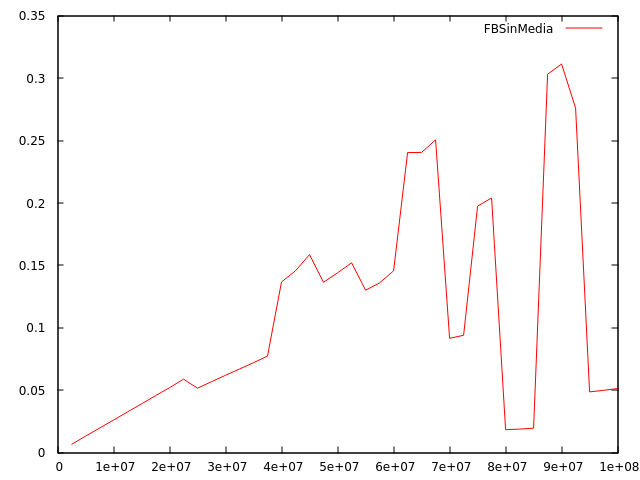
\includegraphics[width=0.6\textwidth]{fbmal.png}
				\caption{Gráfica del algoritmo de fuerza bruta con datos de una única ejecución.}

			\end{figure}

			\par
			Sin embargo, la gráfica es bastante más uniforme al hacer la media de 200 ejecuciones.

			\begin{figure}[h]

				\centering
				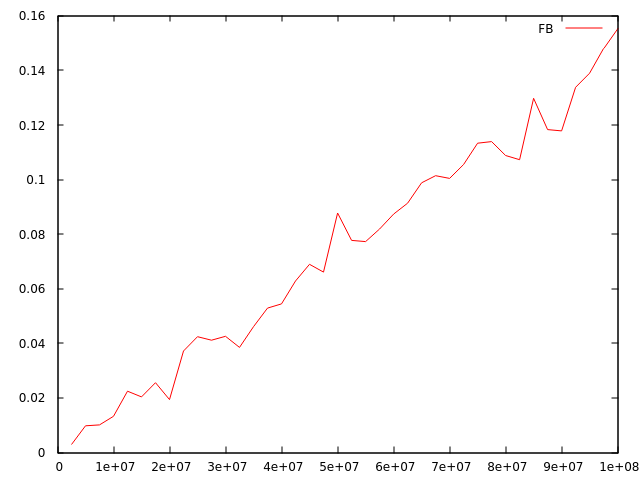
\includegraphics[width=0.6\textwidth]{FB.png}
				\caption{Gráfica del algoritmo de fuerza bruta con la media de los tiempos de ejecución.}

			\end{figure}


\newpage

	\section{Aproximación directa.}

		\subsection{Pseudocódigo.}

			\vspace{0.5cm}

			\begin{algorithm}[H]

				\textbf{function} BusquedaFB(elementos, inicio, fin);

				\Begin{

					solucion $\longleftarrow$ inicio;

					\uIf{tamaño del vector = 2 $and$ primero $<$ segundo}{

						\KwRet segundo;

					}
					\ElseIf{tamaño del vector $>$ 1}{

						\For{$x \in $ elementos}{

							\If{x $ > $ siguiente}{

								\KwRet x;

							}
						}
					}

					\KwRet solucion;

				}

			\end{algorithm}

		\subsection{Código fuente utilizado.}

			\BusquedaFB[label="."]{practica2dyv.cpp}

\newpage

		\subsection{Análisis híbrido.}

			\par
			Como podemos ver en la gráfica, los datos obtenidos se ajustan relativamente bien a la función lineal $f(x) = ax$. 

			\begin{figure}[h]

				\centering
				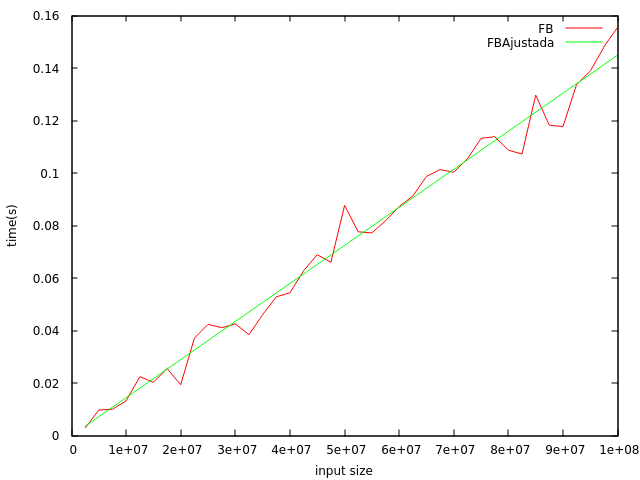
\includegraphics[width=1\textwidth]{FBAjustada.png}
				\caption{Gráfica del algoritmo de fuerza bruta. Compilación sin optimización. Intel® Core™ i7-5500U CPU @ 2.40GHz.}

			\end{figure}

			\par
			El análisis híbrido de los datos representados en la gráfica produce el siguiente resultado:

			\begin{itemize}

				\item
				$a$ $=$ $1.45022\cdot 10^{-9}$

			\end{itemize}

			\par
			$f(x)$ $=$ $ 1.45022\cdot 10^{-9}\cdot x$

			\vspace{5mm}

			\par
			El error en el ajuste es de un $1.051\%$.

\newpage

	\section{Algoritmo \textit{Divide y Vencerás}.}

		\subsection{Pseudocódigo.}

			\begin{algorithm}[H]

				\textbf{function} BusquedaDyV(elementos, inicio, fin);

				\Begin{

					\eIf{tamaño del vector $\leq$ umbral}{

						solucion $\longleftarrow$ BusquedaFB(elementos, inicio, fin);

					}{

						solucion $\longleftarrow$ elemento central;

						\uIf{solucion en secuencia ascendente}{

							solucion $\longleftarrow$ BusquedaDyV(elementos, solucion$+ 1$, fin);

						}
						\ElseIf{solucion en secuencia descendente}{

							solucion $\longleftarrow$ BusquedaDyV(elementos, inicio, solucion);

						}
					}

					\KwRet solucion;

				}

			\end{algorithm}

		\subsection{Código fuente utilizado.}

			\BusquedaDyV[label="."]{practica2dyv.cpp}

\newpage

		\subsection{Análisis híbrido.}

			\par
			En la siguiente gráfica vemos que la curva teórica $f(x) = a \log_{}(x)$ no se corresponde con el comportamiento real del algoritmo a pesar de un error en el ajuste de sólo un $2.01\%$. 

			\begin{figure}[h]

				\centering
				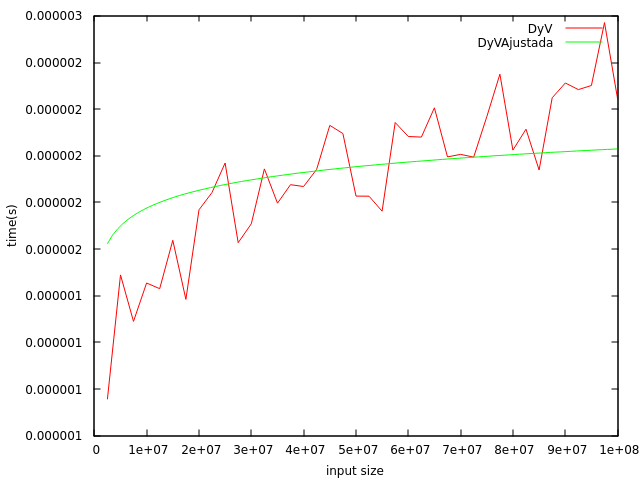
\includegraphics[width=1\textwidth]{DyVAjustada.png}
				\caption{Gráfica del algoritmo \textit{Divide y Vencerás}. Compilación sin optimización. Intel® Core™ i7-5500U CPU @ 2.40GHz.}

			\end{figure}

			\par
			El análisis híbrido de los datos representados en la gráfica produce el siguiente resultado:

			\begin{itemize}

				\item
				$a$ $=$ $1.1017\cdot 10^{-7}$

			\end{itemize}

			\par
			$f(x)$ $=$ $ 1.1017\cdot 10^{-7}\cdot \log_{}(x)$

			\vspace{5mm}

			\par
			El error en el ajuste es de un $2.01\%$.

\newpage

	\section{Comparativa de ambos algoritmos.}

		\subsection{Gráfica de tiempos de ejecución.}

			\par
			A continuación, presentamos una gráfica para observar mejor las diferencias de rendimiento entre los distintos algoritmos:

			\begin{figure}[h]

				\centering
				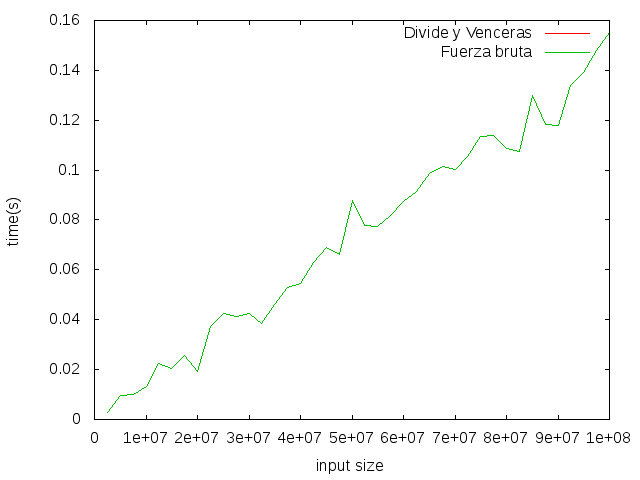
\includegraphics[width=1\textwidth]{comparativa.png}
				\caption{Gráfica comparativa de ambos algoritmos. Compilación sin optimización. Intel® Core™ i7-5500U CPU @ 2.40GHz.}

			\end{figure}

			\vspace{5mm}

			\par
			La diferencia de órdenes de eficiencia de ambos algoritmos impide que los tiempos de ejecución del algoritmo \textit{Divide y Vencerás} aparezcan siquiera en la gráfica. Para hacernos una idea, la diferencia de rendimiento es de un $3084.32\%$ para el tamaño de entrada más pequeño y un $69232.96\%$ para el tamaño de entrada más grande.

\newpage

	\section{Conclusión.}

		\par
		Como hemos podido comprobar, el algoritmo \textit{Divide y Vencerás} tiene tiempos de ejecución mejores que el algoritmo de fuerza bruta. Esto se debe a que, aunque el algoritmo \textit{Divide y Vencerás} consume tiempo dividiendo el problema, sólo analiza la parte en la que sabe que encontrará la solución.		

\end{document}